\documentclass[11pt]{article}
\usepackage[margin=1in]{geometry}
\usepackage{amsmath,amssymb}
\usepackage{enumerate}
\usepackage{array}
\usepackage{tikz}
\usetikzlibrary{trees}
\setlength{\parindent}{0pt}
\setlength{\parskip}{4pt}

\tikzset{
  dec/.style={circle,fill,inner sep=1.6pt},
  gametree/.style={level distance=17mm, every node/.style={font=\small}},
  opt/.style={line width=1.6pt}
}

\title{Problem set 2 \\ \large Solution Key}
\author{Econ 5030}
\date{Due 10/12/26}

\begin{document}
\maketitle

Payoff pairs are written (row player, column player) unless stated otherwise.

%%%%%%%%%%%%%%%%%%%%%%%%%%%%%%%%%%%%%%%%%%%%%%%%%%%%%%%%%%%%%%%%%%%%%%%
\section{Iterated deletion}

\begin{center}
\begin{tabular}{r|ccc}
 & $n_P$ & $l_P$ & $h_P$ \\ \hline
$n_G$ & $0,0$ & $1,2$ & $1,2$ \\
$l_G$ & $3,1$ & $3,3$ & $3,4$ \\
$h_G$ & $2,1$ & $4,3$ & $5,5$
\end{tabular}
\end{center}

\textbf{1.A)} \emph{Round 1.} For Greg, $n_G$ is strictly dominated by $l_G$ ($3>0,\ 3>1,\ 3>1$). For Phil, $n_P$ is strictly dominated by $l_P$ ($2>0,\ 3>1,\ 3>1$). ($h_P$ only \emph{weakly} dominates $l_P$, since $2=2$ against $n_G$, so $l_P$ is not deleted yet.) Delete $n_G$ and $n_P$.

\emph{Round 2.} In the remaining game
\begin{center}
\begin{tabular}{r|cc}
 & $l_P$ & $h_P$ \\ \hline
$l_G$ & $3,3$ & $3,4$ \\
$h_G$ & $4,3$ & $5,5$
\end{tabular}
\end{center}
$h_G$ strictly dominates $l_G$ ($4>3,\ 5>3$) and $h_P$ strictly dominates $l_P$ ($4>3,\ 5>3$). Delete $l_G$ and $l_P$.

Nothing else can be deleted. The solution set is $\{h_G\}\times\{h_P\}$, i.e.\ the profile $(h_G,h_P)$ with payoffs $(5,5)$.

\textbf{1.B)} Best responses:
$BR_G(n_P)=\{l_G\}$, $BR_G(l_P)=\{h_G\}$, $BR_G(h_P)=\{h_G\}$;\quad
$BR_P(n_G)=\{l_P,h_P\}$, $BR_P(l_G)=\{h_P\}$, $BR_P(h_G)=\{h_P\}$.

The only profile where each strategy is a best response to the other is $(h_G,h_P)$. So the set of Nash equilibria is $\{(h_G,h_P)\}$. Since the game is solved by iterated strict dominance, this is also the unique equilibrium in mixed strategies: a strategy that is deleted by iterated strict dominance gets zero probability in every Nash equilibrium.

%%%%%%%%%%%%%%%%%%%%%%%%%%%%%%%%%%%%%%%%%%%%%%%%%%%%%%%%%%%%%%%%%%%%%%%
\section{Putting games into the Normal Form}

\textbf{1. Game tree.} Payoffs are $(u_1,u_2)$. Thick branches are the moves chosen by backward induction (part 5).
\begin{center}
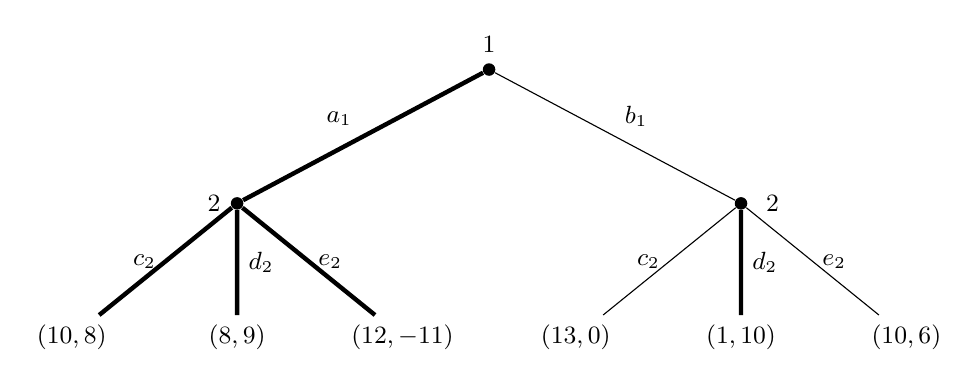
\begin{tikzpicture}[gametree,
  level 1/.style={sibling distance=64mm},
  level 2/.style={sibling distance=21mm}]
\node[dec,label=above:{1}] {}
  child { node[dec,label=left:{2\ }] {}
    child { node {$(10,8)$} edge from parent node[left] {$c_2$} }
    child { node {$(8,9)$} edge from parent[opt] node[right] {$d_2$} }
    child { node {$(12,-11)$} edge from parent node[right] {$e_2$} }
    edge from parent[opt] node[above left] {$a_1$} }
  child { node[dec,label=right:{\ 2}] {}
    child { node {$(13,0)$} edge from parent node[left] {$c_2$} }
    child { node {$(1,10)$} edge from parent[opt] node[right] {$d_2$} }
    child { node {$(10,6)$} edge from parent node[right] {$e_2$} }
    edge from parent node[above right] {$b_1$} };
\end{tikzpicture}
\end{center}

\textbf{2. Strategies.} $S_1=\{a_1,b_1\}$. Player 2 moves at two information sets (after $a_1$ and after $b_1$), so a strategy is a pair $(x,y)$: play $x$ after $a_1$ and $y$ after $b_1$, with $x,y\in\{c_2,d_2,e_2\}$:
\[
S_2=\{c_2c_2,\ c_2d_2,\ c_2e_2,\ d_2c_2,\ d_2d_2,\ d_2e_2,\ e_2c_2,\ e_2d_2,\ e_2e_2\}\quad(3\times3=9\text{ strategies}).
\]

\textbf{3. Normal form} (rows Player 1, columns Player 2; best responses underlined).
\begin{center}
\small
\setlength{\tabcolsep}{4pt}
\begin{tabular}{r|ccccccccc}
 & $c_2c_2$ & $c_2d_2$ & $c_2e_2$ & $d_2c_2$ & $d_2d_2$ & $d_2e_2$ & $e_2c_2$ & $e_2d_2$ & $e_2e_2$ \\ \hline
$a_1$ & $10,8$ & $\underline{10},8$ & $\underline{10},8$ & $8,\underline{9}$ & $\underline{8},\underline{9}$ & $8,\underline{9}$ & $12,-11$ & $\underline{12},-11$ & $\underline{12},-11$ \\
$b_1$ & $\underline{13},0$ & $1,\underline{10}$ & $\underline{10},6$ & $\underline{13},0$ & $1,\underline{10}$ & $\underline{10},6$ & $\underline{13},0$ & $1,\underline{10}$ & $10,6$
\end{tabular}
\end{center}

\textbf{4. Nash equilibria.} Against $a_1$, Player 2's best responses are the strategies with $d_2$ after $a_1$ ($9>8>-11$): $d_2c_2, d_2d_2, d_2e_2$. Against these, $a_1$ gives Player 1 $8$, while $b_1$ gives $13, 1, 10$; only $d_2d_2$ keeps $a_1$ optimal. Against $b_1$, Player 2's best responses have $d_2$ after $b_1$: $c_2d_2, d_2d_2, e_2d_2$. Against these, $b_1$ gives $1$ but $a_1$ gives $10, 8, 12$, so there is no equilibrium with $b_1$.

The unique pure-strategy Nash equilibrium is $(a_1,\ d_2d_2)$, with outcome $(a_1,d_2)$ and payoffs $(8,9)$.

(Mixed strategies: Player 1 cannot mix, because if both $a_1$ and $b_1$ have positive probability Player 2's unique best response is $d_2d_2$, and then $a_1$ is strictly better. With Player 1 playing $a_1$, Player 2 can play $d_2$ after $a_1$ and randomize after $b_1$ with probabilities $(q_c,q_d,q_e)$, provided $13q_c+q_d+10q_e\le 8$. Every such equilibrium has the same outcome $(a_1,d_2)$.)

\textbf{5. Incredible threats?} No. By backward induction Player 2 plays $d_2$ after $a_1$ ($9>8>-11$) and $d_2$ after $b_1$ ($10>6>0$). Player 1 then compares $8$ (from $a_1$) with $1$ (from $b_1$) and plays $a_1$. The subgame perfect equilibrium is $(a_1, d_2d_2)$, which is exactly the unique pure Nash equilibrium. What deters $b_1$ is Player 2's response $d_2$, and $d_2$ is her best move once $b_1$ has been played, so the threat is credible. (In the mixed equilibria above, Player 2's off-path weight on $c_2$ or $e_2$ is not optimal. But those moves would give Player 1 $13$ or $10$, which makes $b_1$ \emph{more} attractive, so they are not threats that hold the equilibrium together.)

%%%%%%%%%%%%%%%%%%%%%%%%%%%%%%%%%%%%%%%%%%%%%%%%%%%%%%%%%%%%%%%%%%%%%%%
\section{Timing and Strategies}

\textbf{2.1 Simultaneous.} Neither player observes the other's choice, so each player has a single information set and a strategy is just an action: $S_1=S_2=\{0,1\}$.
\begin{center}
\begin{tabular}{r|cc}
P1$\backslash$P2 & $0$ & $1$ \\ \hline
$0$ & $1,0$ & $0,1$ \\
$1$ & $0,1$ & $1,0$
\end{tabular}
\end{center}
This is Matching Pennies. There is no pure Nash equilibrium. The unique equilibrium has each player choosing $0$ and $1$ with probability $\tfrac12$, so each expects $\$\tfrac12$.

\textbf{2.2 Sequential.} Player 1 still has $S_1=\{0,1\}$. Player 2 moves after seeing Player 1's choice, so she has two information sets and her strategy must be a complete contingent plan $(x,y)$: play $x$ if Player 1 chose $0$ and $y$ if Player 1 chose $1$:
\[
S_2=\{(0,0),\ (0,1),\ (1,0),\ (1,1)\} = \{\text{always }0,\ \text{copy},\ \text{do the opposite},\ \text{always }1\}.
\]

\textbf{2.3 Difference in the normal forms.} The physical actions are the same, but the strategy sets are not. The simultaneous game is $2\times2$. The sequential game is $2\times4$:
\begin{center}
\begin{tabular}{r|cccc}
P1$\backslash$P2 & $(0,0)$ & $(0,1)$ & $(1,0)$ & $(1,1)$ \\ \hline
$0$ & $1,0$ & $1,0$ & $0,1$ & $0,1$ \\
$1$ & $0,1$ & $1,0$ & $0,1$ & $1,0$
\end{tabular}
\end{center}
Timing and information enter the normal form only through the strategy sets. Because Player 2 can condition on what she sees, she has more strategies, and some payoff columns repeat. This changes the predictions. In the sequential game the strategy $(1,0)$ (do the opposite) wins for Player 2 against anything. The Nash equilibria are Player 2 playing $(1,0)$ with Player 1 playing anything; in pure strategies these are $(0,(1,0))$ and $(1,(1,0))$, with payoffs $(0,1)$. In the simultaneous game each player wins with probability $\tfrac12$. The $2\times4$ matrix would also describe a simultaneous game in which Player 2 submits a contingent plan in advance, so the normal form records information only through what strategies can condition on.

%%%%%%%%%%%%%%%%%%%%%%%%%%%%%%%%%%%%%%%%%%%%%%%%%%%%%%%%%%%%%%%%%%%%%%%
\section{Third party observation of a game}

\textbf{2.4} No, not by itself. If each player's payoff were her own money, $(M_1,M_2)$ would not be a Nash equilibrium: holding the opponent at $M$, a player gains by deviating. The table does not label whose dollar amount comes first, but the conclusion holds under either reading:
\begin{itemize}
\item First entry = row player (Player 2). Against $M$, switching to $L$ pays $\$30>\$18$. The money game's equilibria are $(L_1,M_2)$, $(M_1,L_2)$, and a mixed equilibrium with each player choosing $L$ with probability $6/7$ and $M$ with probability $1/7$.
\item First entry = Player 1. Against $M$, switching to $H$ pays $\$20>\$18$. Here $L$ is strictly dominated by $M$, and once $L$ is deleted, $M$ is strictly dominated by $H$, so the unique equilibrium is $(H_1,H_2)$ with $\$5$ each.
\end{itemize}
So the data reject the joint hypothesis that players maximize their \emph{own money} and play a Nash equilibrium. They do not reject game theory. In a game, payoffs are utilities that represent each player's preferences over outcomes. The experimenter controls the money but not the preferences, and if players care about more than their own earnings, the game they are actually playing has different payoffs from the money table. Universal $M$ play is consistent with Nash play of such a game (2.6).

\textbf{2.5 Normal form.} A normal-form game is $G=(N,\{S_i\}_{i\in N},\{u_i\}_{i\in N})$, where:
\begin{itemize}
\item $N$ is the set of players;
\item $S_i$ is Player $i$'s set of strategies, where a strategy is a complete contingent plan specifying an action at every point where $i$ might move, including points that are never reached;
\item $u_i:S\to\mathbb{R}$, with $S=\prod_j S_j$, gives $i$'s payoff from each strategy profile. It is a utility representation of $i$'s preferences over the outcome the profile produces. It is ordinal for pure-strategy analysis, and once mixed strategies or beliefs are involved it must be a von Neumann--Morgenstern utility.
\end{itemize}
The normal form treats players as choosing whole strategies simultaneously and independently. Timing and information are not shown directly; they show up only through what the strategies can condition on. In this experiment $N=\{1,2\}$ and $S_i=\{L_i,M_i,H_i\}$, but $u_i$ is the utility a player gets from the money pair, which need not equal her own money.

\textbf{2.6 Explanation and game.} Postulate social (fairness) preferences: each subject values the pair's total earnings and puts extra weight on the worse-off subject's earnings (Charness--Rabin-style social-welfare preferences):
\[
u_i(x_1,x_2)=x_1+x_2+\min\{x_1,x_2\}.
\]
Because $u_i$ is symmetric in $(x_1,x_2)$, both players get the same utility in each cell, whichever way the money table is read. The normal form is
\begin{center}
\begin{tabular}{r|ccc}
 & $L_1$ & $M_1$ & $H_1$ \\ \hline
$L_2$ & $24,24$ & $50,50$ & $17,17$ \\
$M_2$ & $50,50$ & $\mathbf{54,54}$ & $28,28$ \\
$H_2$ & $17,17$ & $28,28$ & $15,15$
\end{tabular}
\end{center}
For each player $M$ strictly dominates both $L$ and $H$: against $L$, $50>24$ and $50>17$; against $M$, $54>50$ and $54>28$; against $H$, $28>17$ and $28>15$. Iterated deletion leaves only $(M_1,M_2)$, so it is the unique Nash equilibrium, in pure or mixed strategies. This matches the data.

\textbf{Can these data test rationality?} Not on their own. Rationality means choosing a best response under \emph{some} complete, transitive preferences (and beliefs). The experimenter observes money and choices but not utilities. As 2.6 shows, any observed profile can be made the unique (even dominant-strategy) equilibrium by choosing preferences suitably, so choices in a single game cannot refute rationality. They only test rationality \emph{jointly} with an assumed utility function (for example, ``own money only'') and equilibrium beliefs. A real test needs restrictions that tie preferences together across situations. For example, vary the payoffs across many games and check whether one stable utility function explains all the choices (a revealed-preference consistency test), or elicit beliefs and preferences separately.

%%%%%%%%%%%%%%%%%%%%%%%%%%%%%%%%%%%%%%%%%%%%%%%%%%%%%%%%%%%%%%%%%%%%%%%
\section{Subgame Perfect Nash Equilibrium}

(I read the timing as: Player 2 observes Player 1's action and then chooses from $\{U_2,D_2\}$, as the subscripts indicate.)

\textbf{1. Normal form.} $N=\{1,2\}$, $S_1=\{L_1,M_1,H_1\}$. Player 2 has three information sets, so $S_2=\{U_2,D_2\}^3$, with $2^3=8$ strategies $(x_L,x_M,x_H)$, where $x_k$ is her action after $k_1$. Payoffs are $u_i(s_1,s_2)=u_i(s_1,x_{s_1})$.

\textbf{2. Matrix and Nash equilibria} (strategies written $x_Lx_Mx_H$; best responses underlined).
\begin{center}
\small
\setlength{\tabcolsep}{4pt}
\begin{tabular}{r|cccccccc}
 & $UUU$ & $UUD$ & $UDU$ & $UDD$ & $DUU$ & $DUD$ & $DDU$ & $DDD$ \\ \hline
$L_1$ & $\underline{10},10$ & $\underline{10},10$ & $\underline{10},10$ & $\underline{10},10$ & $1,\underline{11}$ & $1,\underline{11}$ & $1,\underline{11}$ & $1,\underline{11}$ \\
$M_1$ & $5,5$ & $5,5$ & $2,\underline{6}$ & $2,\underline{6}$ & $\underline{5},5$ & $\underline{5},5$ & $\underline{2},\underline{6}$ & $2,\underline{6}$ \\
$H_1$ & $1,4$ & $3,\underline{5}$ & $1,4$ & $3,\underline{5}$ & $1,4$ & $3,\underline{5}$ & $1,4$ & $\underline{3},\underline{5}$
\end{tabular}
\end{center}
Player 2 strictly prefers $D_2$ after every action ($11>10$, $6>5$, $5>4$), so in equilibrium she plays $D_2$ at the node that is reached.
\begin{itemize}
\item $L_1$: Player 2 must play $D$ after $L$, so Player 1 gets $1$, but $M_1$ gives at least $2$. No equilibrium.
\item $M_1$: needs $x_M=D$; $x_L=D$ (else $L_1$ gives $10>2$); $x_H=U$ (else $H_1$ gives $3>2$). This gives $(M_1, DDU)$.
\item $H_1$: needs $x_H=D$; $x_L=D$ (else $10>3$); $x_M=D$ (else $5>3$). This gives $(H_1, DDD)$.
\end{itemize}
The pure-strategy Nash equilibria are $(M_1,\ D_2D_2U_2)$ with payoffs $(2,6)$ and $(H_1,\ D_2D_2D_2)$ with payoffs $(3,5)$.

(Mixed strategies: Player 1 never mixes in equilibrium. There are also mixed versions of each equilibrium that differ only off the path. With the outcome $(M_1,D_2)$: Pr$(U\mid L)\le 1/9$ and Pr$(U\mid H)\ge 1/2$. With the outcome $(H_1,D_2)$: Pr$(U\mid L)\le 2/9$ and Pr$(U\mid M)\le 1/3$.)

\textbf{3. Game tree and SPE.} Payoffs are $(u_1,u_2)$. Thick branches are the backward-induction choices.
\begin{center}
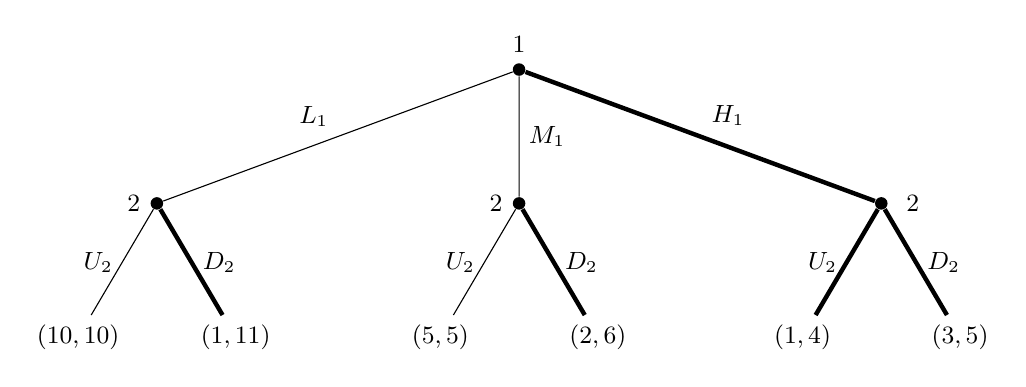
\begin{tikzpicture}[gametree,
  level 1/.style={sibling distance=46mm},
  level 2/.style={sibling distance=20mm}]
\node[dec,label=above:{1}] {}
  child { node[dec,label=left:{2\ }] {}
    child { node {$(10,10)$} edge from parent node[left] {$U_2$} }
    child { node {$(1,11)$} edge from parent[opt] node[right] {$D_2$} }
    edge from parent node[above left] {$L_1$} }
  child { node[dec,label=left:{2\ }] {}
    child { node {$(5,5)$} edge from parent node[left] {$U_2$} }
    child { node {$(2,6)$} edge from parent[opt] node[right] {$D_2$} }
    edge from parent node[right] {$M_1$} }
  child { node[dec,label=right:{\ 2}] {}
    child { node {$(1,4)$} edge from parent node[left] {$U_2$} }
    child { node {$(3,5)$} edge from parent[opt] node[right] {$D_2$} }
    edge from parent[opt] node[above right] {$H_1$} };
\end{tikzpicture}
\end{center}
Backward induction: in each of the three subgames Player 2 plays $D_2$ ($11>10$, $6>5$, $5>4$). Anticipating this, Player 1 gets $1$, $2$, $3$ from $L_1$, $M_1$, $H_1$ and chooses $H_1$.

The unique subgame perfect Nash equilibrium is $(H_1,\ D_2D_2D_2)$, with outcome $(H_1,D_2)$ and payoffs $(3,5)$. The other Nash equilibrium $(M_1, D_2D_2U_2)$ is not subgame perfect. It rests on the incredible threat to play $U_2$ after $H_1$, which Player 2 would not carry out because it gives her $4<5$.

\end{document}
